\section{Chess theorem}

\begin{theorem}[Von Neumann]
    In the game of chess, one and only one of the following alternatives holds:
\end{theorem}
\begin{enumerate}
    \item \textit{The White has a way to win, no matter what the Black does.}
    \item \textit{White has a strategy to guarantee a win, regardless of what Black does.}
    \item \textit{Both White and Black can force at least a draw, regardless of the opponent's actions.}
\end{enumerate}

\begin{proof}
    Assume the game has a finite length of $2K$ moves, where each player makes $K$ moves. 
    Let $a_i$ represent White's move at their $i$-th stage, and $b_i$ represent Black's corresponding move. 

    The first possibility in the theorem can be formulated as follows:
    \[\exists a_1 : \forall b_1 \exists a_2 : \forall b_2 \dots \exists a_K : \forall b_K \implies \text{white wins}\]
    Now, suppose this is false. 
    Then the negation is:
    \[\forall a_1 \exists b_1 : \forall a_2 : \exists b_2 : \dots \forall a_K : \exists b_K \implies \text{white does not win}\]
    This means Black has the possibility to prevent White from winning, ensuring at least a draw.
    
    If White does not have a winning strategy, then Black can secure at least a draw. 
    Similarly, if Black does not have a winning strategy, then White can secure at least a draw. 
    Therefore, if neither of the first two possibilities holds, the third one must be true.
\end{proof}

\subsection{Extension}
Von Neumann's theorem can be extended to any finite game of perfect information where the possible outcomes are either a win for one player or a tie. 
\begin{corollary}
    Consider a finite, perfect information game with two players, where the only possible outcomes are a win for one of the players or a tie. 
    Then, exactly one of the following holds:
\end{corollary}
\begin{enumerate}
    \item \textit{Player 1 has a winning strategy, no matter what the second player does.}
    \item \textit{Player 2 has a winning strategy, no matter what the second player does.}
\end{enumerate}
The possible solutions for a game are classified as follows:
\begin{itemize}
    \item \textit{Very weak solution}: the game has a rational outcome, but it is not accessible in practice, as with chess.
    \item \textit{Weak solution}: the outcome of the game is known, but the method to achieve it is not generally understood.
    \item \textit{Solution}: there exists an algorithm that can determine the outcome.
\end{itemize}












\begin{example}
    Consider the game of chomp.
    In this game we have a grid in which each player can remove a tile with all the others on the right and above it. 
    In this game we have a solution if the grid is a square, and a weak solution if the grid is rectangular.
    In the latter case we may have the following situation: 
    \begin{figure}[H]
        \centering
        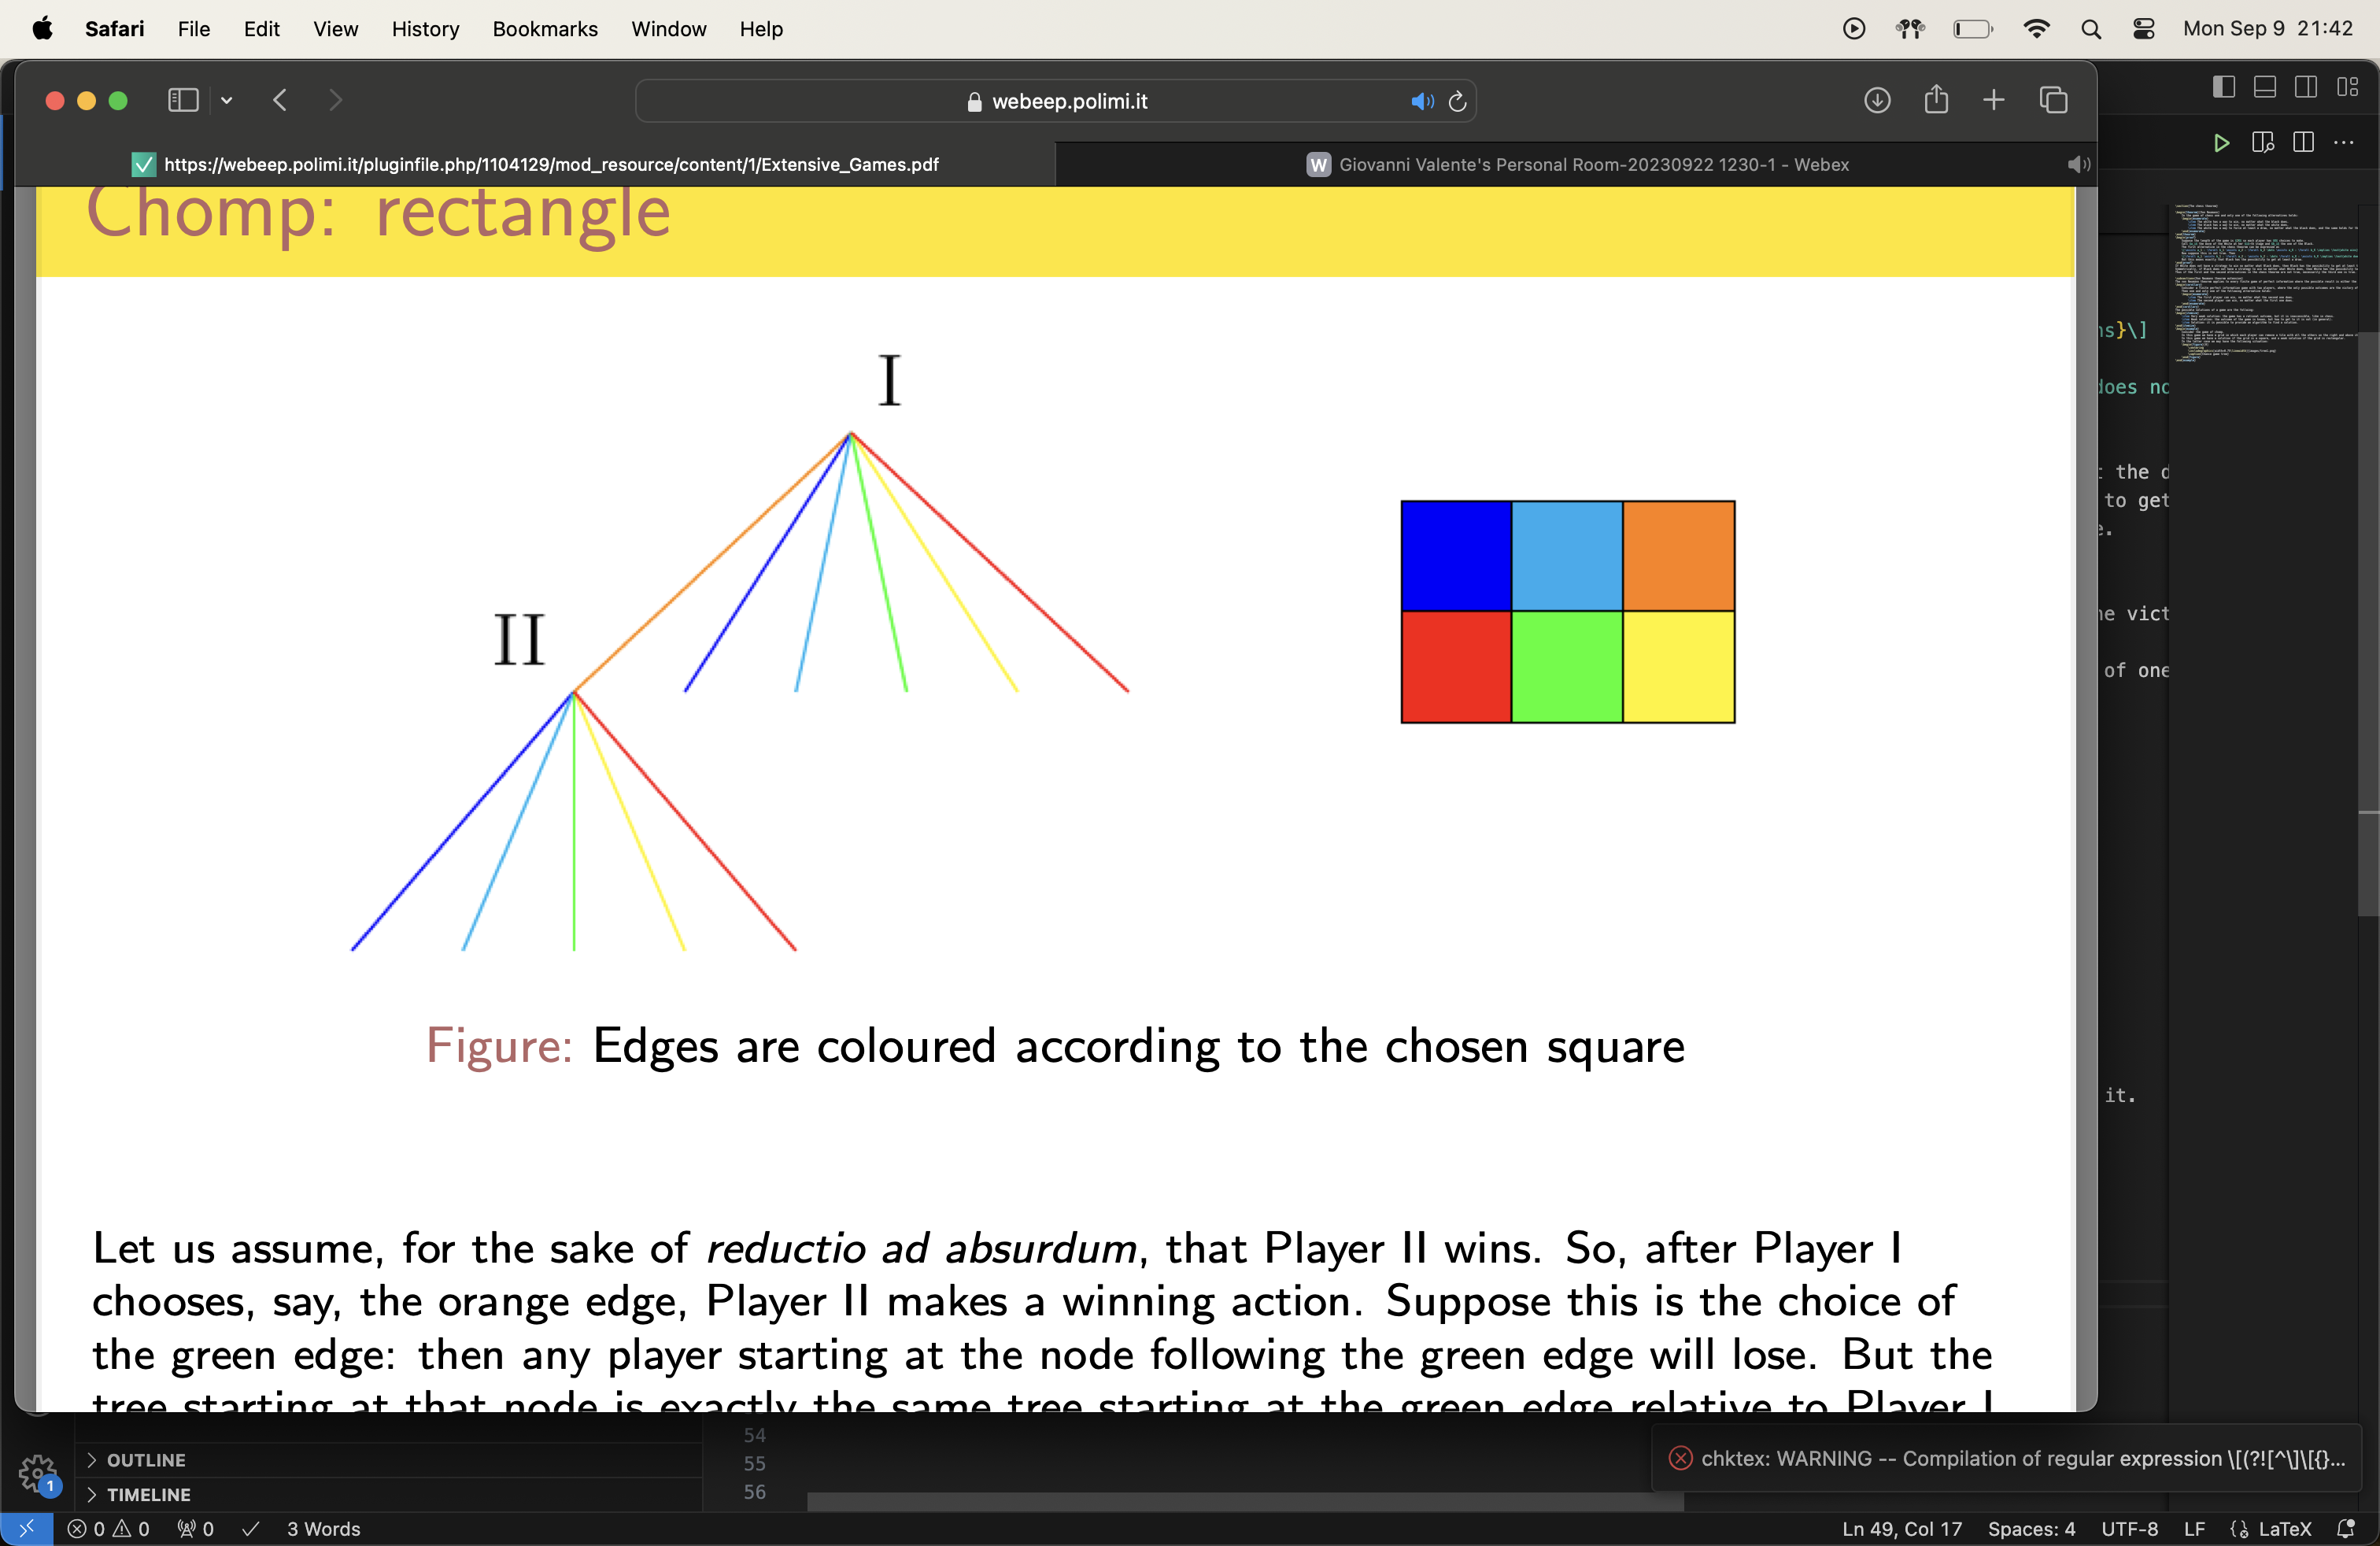
\includegraphics[width=0.75\linewidth]{images/chomp.png}
        \caption{Rectangular chomp}
    \end{figure}
    Let us assume, for the sake of reductio ad absurdum, that Player II wins. So, after Player I
    chooses, say, the orange edge, Player II makes a winning action. Suppose this is the choice of
    the green edge: then any player starting at the node following the green edge will lose. But the
    tree starting at that node is exactly the same tree starting at the green edge relative to Player I.
    Thus Player I has a move available that guarantees victory, whereby Player II would have to lose.
    Since we derived a contradiction, the original assumption must be false: it is Player I that wins!
\end{example}







